\documentclass[aspectratio=169,10pt]{beamer}
\usepackage[T1]{fontenc}
\usepackage[utf8]{inputenc}
% babel indisponível neste ambiente; no seu LaTeX use \usepackage[brazil]{babel}
\renewcommand{\proofname}{Prova}
\usepackage{amsmath,amssymb,amsthm}
\usepackage{tikz}
\usetikzlibrary{shapes.geometric,arrows.meta,positioning,decorations.pathreplacing}
\usepackage{algpseudocode}

\usetheme{Madrid}
\setbeamertemplate{navigation symbols}{}
\setbeamertemplate{footline}[frame number]
\setbeamertemplate{enumerate items}[default]
\setbeamerfont{block title}{size=\small}

% ---------- macros ----------
\newcommand{\Cria}{\mathtt{cria}}
\newcommand{\Busca}{\mathtt{busca}}
\newcommand{\Uniao}{\mathtt{uniao}}
\newcommand{\Link}{\mathtt{link}}
\renewcommand{\lg}{\operatorname{lg}}
\newcommand{\lgs}{\lg^{*}}
\tikzset{>=Stealth}

% ---------- pseudocódigo em português ----------
\algrenewcommand\algorithmicrequire{\textbf{Entrada:}}
\algrenewcommand\algorithmicwhile{\textbf{enquanto}}
\algrenewcommand\algorithmicdo{\textbf{faça}}
\algrenewcommand\algorithmicfor{\textbf{para}}
\algrenewcommand\algorithmicforall{\textbf{para cada}}
\algrenewcommand\algorithmicif{\textbf{se}}
\algrenewcommand\algorithmicthen{\textbf{então}}
\algrenewcommand\algorithmicelse{\textbf{senão}}
\algrenewcommand\algorithmicend{\textbf{fim}}
\algrenewcommand\algorithmicreturn{\textbf{devolva}}
\algrenewcommand\alglinenumber[1]{\scriptsize #1:}
\algrenewcommand\algorithmiccomment[1]{\hfill$\triangleright$ #1}

\title[Conjuntos disjuntos]{Estruturas de dados para conjuntos disjuntos}
\subtitle{Ideias e intuição por trás das análises}
\author{Jair}
\institute{CMCC -- UFABC}
\date{}


\begin{document}

\begin{frame}[plain]
  \titlepage
\end{frame}

% ===================================================================
\begin{frame}[t]{Para onde vamos}
  \small
  Queremos manter uma partição de $\{1,\dots,n\}$ com três operações:
  $\Cria$, $\Busca$ (quem é o representante do meu conjunto?) e
  $\Uniao$ (junte dois conjuntos).

  \medskip
  Compararemos quatro estruturas pelo \textbf{tempo total de $m$
    operações}, e não pelo pior caso de cada uma.

  \medskip
  \begin{center}
    \renewcommand{\arraystretch}{1.3}
    \begin{tabular}{|l|l|}\hline
      \textbf{estrutura} & \textbf{ideia em uma frase}\\\hline
      vetor & cada elemento guarda o nome do seu conjunto; unir é
      \textit{renomear}\\\hline
      listas ligadas & renomear só o conjunto \textbf{menor}\\\hline
      floresta & unir é pendurar uma árvore em outra; buscar é
      \textit{subir}\\\hline
      floresta + rank + compressão & subir também \textbf{achata} a árvore\\\hline
    \end{tabular}
  \end{center}

  \medskip
  Motivação: o algoritmo de Kruskal.
\end{frame}

% ===================================================================
\begin{frame}[t]{Kruskal: por que conjuntos disjuntos?}
  \small
  Enquanto o Kruskal roda, $(V,S)$ é uma floresta; seus componentes
  formam uma \textbf{partição} de $V$.

  \medskip
  \begin{block}{A observação-chave}
    Uma aresta $\{x,y\}$ pode ser inserida sem criar circuito
    $\iff$ $x$ e $y$ estão em \textbf{componentes diferentes}.
  \end{block}
  \textit{Por quê?}  Se estão no mesmo componente, já há um caminho
  entre eles, e a aresta o fecha num circuito.  Se estão em componentes
  diferentes, não há caminho entre eles, e qualquer circuito novo teria
  que passar pela aresta e voltar por um caminho que não existe.

  \medskip
  Então o Kruskal só precisa de: \textit{``$x$ e $y$ estão no mesmo
    conjunto?''} (duas buscas) e \textit{``junte os dois conjuntos''}
  (uma união).
\end{frame}

\begin{frame}[t]{Kruskal com conjuntos disjuntos}
  \footnotesize
  \begin{minipage}[t]{.52\linewidth}
    \begin{algorithmic}[1]
      \Require grafo conexo $G=(V,E)$ com pesos nas arestas
      \State $S\gets\emptyset$
      \State $F\gets$ lista das arestas em ordem crescente de peso
      \ForAll{$v\in V$}
      \State $\Cria(v)$
      \EndFor
      \ForAll{$\{u,v\}\in F$}
      \If{$\Busca(u)\neq\Busca(v)$}
      \State insira $\{u,v\}$ em $S$
      \State $\Uniao(u,v)$
      \EndIf
      \EndFor
      \State \Return $(V,S)$
    \end{algorithmic}
  \end{minipage}
  \hfill
  \begin{minipage}[t]{.44\linewidth}
    \textbf{Contagem das operações}
    \begin{itemize}
    \item $|V|$ operações $\Cria$;
    \item no máximo $2|E|$ operações $\Busca$;
    \item no máximo $|V|-1$ operações $\Uniao$.
    \end{itemize}
    Total: menos que $2(|E|+|V|)=O(|E|)$, pois $G$ é conexo e
    $|V|\leq|E|+1$.
  \end{minipage}

  \smallskip
  \footnotesize
  \begin{block}{Consequência}
    Com $m=O(|E|)$ operações, o custo do Kruskal é
    \[
      O(|E|\log|E|)\ \ (\text{ordenação})\;+\;\text{custo de }m\text{ operações}.
    \]
    Como $|E|\leq|V|^2$, $O(|E|\log|E|)=O(|E|\log|V|)$.  A estrutura
    escolhida decide se a ordenação domina.
  \end{block}
\end{frame}

% ===================================================================
\begin{frame}[t]{Vetor: unir é renomear}
  \small
  \textbf{Ideia:} cada elemento guarda o \textit{nome} do seu conjunto
  (o menor elemento dele).  Dois elementos estão juntos se e só se têm o
  mesmo nome.
  \begin{itemize}
  \item $\Busca(x)$: ler o nome de $x$ --- $O(1)$.
  \item $\Uniao(x,y)$: \textbf{varrer o vetor inteiro} e trocar o nome
    dos dois conjuntos pelo menor deles --- $\Theta(n)$.
  \end{itemize}

  \medskip
  \begin{alertblock}{Custo}
    Cada união varre $n$ posições e há no máximo $n-1$ uniões, logo
    $m$ operações custam $O(m+n^2)$.  No Kruskal:
    $O(|E|\log|E|+|V|^2)$, que em grafos esparsos é dominado por $|V|^2$.
  \end{alertblock}

  \medskip
  \textbf{O desperdício:} para unir um conjunto minúsculo com um
  enorme, renomeamos \textit{todos} os elementos, inclusive os que já
  estavam certos.
\end{frame}

% ===================================================================
\begin{frame}[t]{Listas ligadas: renomear só o menor}
  \small
  \textbf{Ideia:} cada conjunto é uma lista; cada nó aponta para o
  representante ($\mathtt{rep}$).
  \begin{itemize}
  \item $\Busca(x)$: seguir $\mathtt{rep}$ --- $O(1)$.
  \item $\Uniao(x,y)$: \textbf{percorrer a lista menor}, apontando seus
    nós para o representante da maior, e concatenar --- custo
    proporcional ao tamanho da menor.
  \end{itemize}

  \medskip
  \begin{block}{Heurística $(\ddag)$}
    Numa união, atualize sempre os ponteiros da \textbf{menor} lista.
  \end{block}

  \medskip
  Sem $(\ddag)$ podemos gastar $\Theta(n^2)$ (sempre renomear a lista
  maior); com $(\ddag)$ a análise a seguir mostra $O(m+n\log n)$.
\end{frame}

% ===================================================================
\begin{frame}[t]{Listas ligadas: quem paga a atualização?}
  \small
  Olhe a história de \textbf{um elemento} $x$.  Ele só tem o seu ponteiro
  atualizado quando está na lista \textbf{menor}, e então passa a estar
  numa lista \textbf{pelo menos duas vezes maior}:

  \medskip
  \centering
  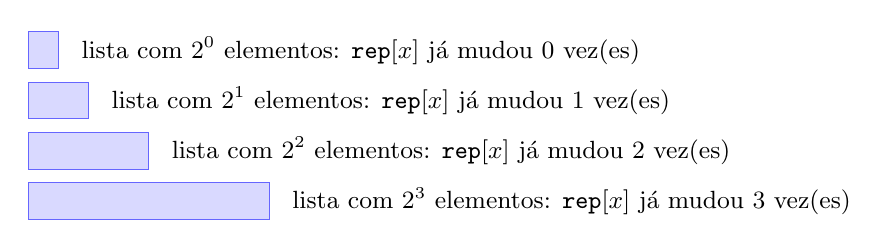
\begin{tikzpicture}[scale=.85]
    \foreach \i in {0,1,2,3} {
      \pgfmathsetmacro{\w}{0.45*(2^\i)}
      \draw[fill=blue!15,draw=blue!60] (0,-0.75*\i) rectangle (\w,-0.75*\i+0.55);
      \node[anchor=west,font=\small] at (\w+0.2,-0.75*\i+0.27)
        {lista com $2^{\i}$ elementos: $\mathtt{rep}[x]$ já mudou $\i$ vez(es)};
    }
  \end{tikzpicture}

  \medskip
  \raggedright
  Como nenhuma lista passa de $n$ elementos, $x$ é atualizado no máximo
  $\log_2 n$ vezes.  \textbf{Cada um dos $n$ elementos paga no máximo
    $\log_2 n$}; o resto das operações custa $O(1)$.

  \begin{block}{Resultado}
    $m$ operações custam $O(m+n\log n)$; o Kruskal fica
    $O(|E|\log|V|)$.  (A prova formal está no apêndice.)
  \end{block}
\end{frame}

% ===================================================================
\begin{frame}[t]{Floresta: cada conjunto é uma árvore}
  \small
  \textbf{Ideia:} em vez de avisar \textit{todos} os elementos, avise só
  a raiz.  Cada elemento aponta para o pai; a raiz é o representante.
  \begin{itemize}
  \item $\Uniao$: pendurar uma raiz na outra --- $O(1)$ depois de achar
    as raízes.
  \item $\Busca(x)$: \textbf{subir} até a raiz --- custa a profundidade
    de $x$.
  \end{itemize}

  \centering
  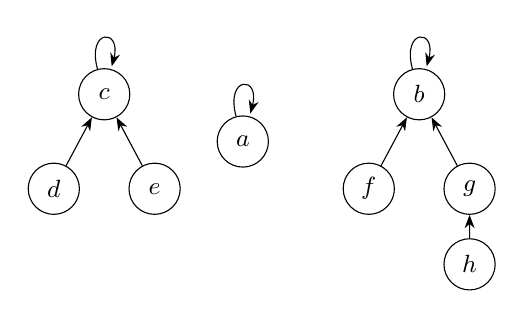
\begin{tikzpicture}[scale=.8,
      vertice/.style={circle, draw, minimum size=6.5mm, inner sep=0pt, font=\small},
      every edge/.style={draw, ->}]
    \node[vertice] (c) at (0, 1.5) {$c$};
    \path (c) edge [loop above] (c);
    \node[vertice] (d) at (-0.8, 0) {$d$};
    \node[vertice] (e) at (0.8, 0) {$e$};
    \draw[->] (d) -- (c);  \draw[->] (e) -- (c);
    \node[vertice] (a) at (2.2, 0.75) {$a$};
    \path (a) edge [loop above] (a);
    \node[vertice] (b) at (5.0, 1.5) {$b$};
    \path (b) edge [loop above] (b);
    \node[vertice] (f) at (4.2, 0) {$f$};
    \node[vertice] (g) at (5.8, 0) {$g$};
    \node[vertice] (h) at (5.8, -1.2) {$h$};
    \draw[->] (f) -- (b);  \draw[->] (g) -- (b);  \draw[->] (h) -- (g);
  \end{tikzpicture}

  {\footnotesize Os conjuntos $\{c,d,e\}$, $\{a\}$ e $\{b,f,g,h\}$.}
\end{frame}

% ===================================================================
\begin{frame}[t]{Floresta: o risco e o remédio}
  \small
  \begin{minipage}[c]{.48\linewidth}
    \centering
    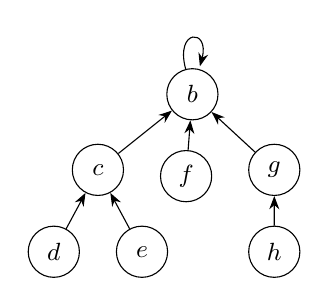
\begin{tikzpicture}[scale=.8,
        vertice/.style={circle, draw, minimum size=6.5mm, inner sep=0pt, font=\small},
        every edge/.style={draw, ->}]
      \node[vertice] (b) at (0, 2) {$b$};
      \path (b) edge [loop above] (b);
      \node[vertice] (c) at (-1.5, 0.8) {$c$};
      \node[vertice] (f) at (-0.1, 0.7) {$f$};
      \node[vertice] (g) at (1.3, 0.8) {$g$};
      \node[vertice] (d) at (-2.2, -0.5) {$d$};
      \node[vertice] (e) at (-0.8, -0.5) {$e$};
      \node[vertice] (h) at (1.3, -0.5) {$h$};
      \draw[->] (d) -- (c);  \draw[->] (e) -- (c);  \draw[->] (c) -- (b);
      \draw[->] (f) -- (b);  \draw[->] (h) -- (g);  \draw[->] (g) -- (b);
    \end{tikzpicture}

    {\footnotesize $\Uniao(e,f)$: a raiz $c$ (tamanho $3$) é pendurada
      na raiz $b$ (tamanho $4$).}
  \end{minipage}
  \hfill
  \begin{minipage}[c]{.48\linewidth}
    \textbf{Risco:} pendurar sempre a árvore \textit{grande} numa
    unitária cria uma cadeia de $n$ nós; uma busca custa $\Theta(n)$.
  \end{minipage}

  \bigskip
  \begin{block}{Remédio: pendurar a menor na maior}
    Por \textbf{tamanho} (número de nós) ou por \textbf{altura}: quem
    é pendurado fica um nível mais fundo, então queremos que seja a
    árvore que ``tem menos a perder''.
  \end{block}
\end{frame}

\begin{frame}[t]{Floresta: algoritmos com união por tamanho}
  \footnotesize
  Cada nó tem $\mathrm{pai}[x]$ e, nas raízes, $t[x]$ = número de
  elementos da árvore enraizada em $x$.

  \medskip
  \begin{minipage}[t]{.3\linewidth}
    \textbf{cria$(x)$}
    \begin{algorithmic}[1]
      \State $\mathrm{pai}[x]\gets x$
      \State $t[x]\gets1$
    \end{algorithmic}
  \end{minipage}
  \hfill
  \begin{minipage}[t]{.33\linewidth}
    \textbf{busca$(x)$}
    \begin{algorithmic}[1]
      \While{$x\neq\mathrm{pai}[x]$}
      \State $x\gets\mathrm{pai}[x]$
      \EndWhile
      \State \Return $x$
    \end{algorithmic}
  \end{minipage}
  \hfill
  \begin{minipage}[t]{.3\linewidth}
    \textbf{link$(x,y)$}
    \begin{algorithmic}[1]
      \State $t[x]\gets t[x]+t[y]$
      \State $\mathrm{pai}[y]\gets x$
    \end{algorithmic}
  \end{minipage}

  \medskip
  $\Link$ pressupõe que $x$ e $y$ são raízes distintas com
  $t[x]\geq t[y]$ (garantido por $\Uniao$); $\Uniao$ pressupõe que $x$ e
  $y$ estão em árvores distintas.

  \medskip
  \textbf{uniao$(x,y)$}
  \begin{algorithmic}[1]
    \State $r_x\gets\Busca(x)$;\ \ $r_y\gets\Busca(y)$
    \If{$t[r_x]\geq t[r_y]$} \State $\Link(r_x,r_y)$
    \Else\ \State $\Link(r_y,r_x)$
    \EndIf
  \end{algorithmic}
\end{frame}

% ===================================================================
\begin{frame}[c]{Floresta: por que a altura fica pequena?}
  \small
  \textbf{Ideia:} a altura de uma árvore só aumenta quando pendurada
  uma árvore de \textit{mesma altura}.  Portanto, uma árvore de altura
  $h$ foi montada a partir de \textbf{duas de altura $h-1$}:

  \medskip
  \centering
  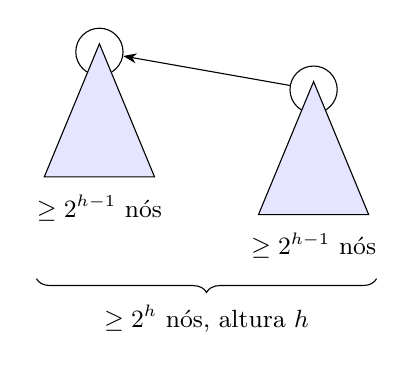
\begin{tikzpicture}[scale=.8,
      vertice/.style={circle,draw,minimum size=6mm,inner sep=0pt,font=\small},
      subtree/.style={isosceles triangle,draw,shape border rotate=90,
        minimum width=14mm,minimum height=11mm,inner sep=0pt,fill=blue!10}]
    \node[vertice] (r) at (0,2.4) {};
    \node[vertice] (s) at (3.4,1.8) {};
    \node[subtree] (A) at (0,1.0) {};
    \node[subtree] (B) at (3.4,0.4) {};
    \draw[->] (s) -- (r);
    \node[font=\small,below=1mm of A] {$\geq2^{h-1}$ nós};
    \node[font=\small,below=1mm of B] {$\geq2^{h-1}$ nós};
    \draw[decorate,decoration={brace,mirror,amplitude=5pt}] (-1,-1.2) -- (4.4,-1.2)
      node[midway,below=6pt,font=\small] {$\geq2^{h}$ nós, altura $h$};
  \end{tikzpicture}

  \smallskip
  \raggedright
  Logo uma árvore de altura $h$ tem $\geq2^h$ nós; com no máximo $n$
  nós, a altura é $\leq\log_2n$.  Cada $\Busca$ custa $O(\log n)$ e
  \begin{block}{Resultado}
    $m$ operações custam $O(m(1+\log n))$; o Kruskal fica
    $O(|E|\log|V|)$.
  \end{block}
\end{frame}

% ===================================================================
\begin{frame}[t]{Compressão de caminhos: subir também arruma}
  \small
  \textbf{Ideia:} uma busca já percorreu o caminho de $x$ até a raiz;
  aproveitamos a viagem e fazemos \textbf{todos os nós do caminho
    apontarem direto para a raiz}.  A próxima busca por qualquer um
  deles custa $O(1)$.

  \centering
  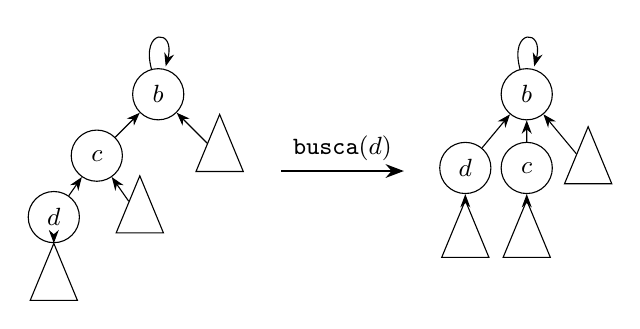
\begin{tikzpicture}[scale=.78,
      vertice/.style={circle, draw, minimum size=6.5mm, inner sep=0pt, font=\small},
      subtree/.style={isosceles triangle, draw, shape border rotate=90,
        minimum width=6mm, minimum height=7mm, inner sep=0pt},
      every edge/.style={draw, ->}]
    \node[vertice] (b1) at (0, 2.5) {$b$};
    \path (b1) edge [loop above] (b1);
    \node[vertice] (c1) at (-1, 1.5) {$c$};
    \node[vertice] (d1) at (-1.7, 0.5) {$d$};
    \node[subtree] (s11) at (-1.7, -0.6) {};
    \node[subtree] (s12) at (-0.3, 0.5) {};
    \node[subtree] (s13) at (1, 1.5) {};
    \draw[->] (s11) -- (d1);  \draw[->] (d1) -- (c1);
    \draw[->] (s12) -- (c1);  \draw[->] (c1) -- (b1);  \draw[->] (s13) -- (b1);
    \draw[->, thick] (2, 1.25) -- (4, 1.25)
      node[midway, above, font=\small] {$\Busca(d)$};
    \node[vertice] (b2) at (6, 2.5) {$b$};
    \path (b2) edge [loop above] (b2);
    \node[vertice] (c2) at (6, 1.3) {$c$};
    \node[vertice] (d2) at (5, 1.3) {$d$};
    \node[subtree] (s21) at (5, 0.1) {};
    \node[subtree] (s22) at (6, 0.1) {};
    \node[subtree] (s23) at (7, 1.3) {};
    \draw[->] (s21) -- (d2);  \draw[->] (d2) -- (b2);
    \draw[->] (s22) -- (c2);  \draw[->] (c2) -- (b2);  \draw[->] (s23) -- (b2);
  \end{tikzpicture}

  \raggedright\small
  \medskip
  Uma busca \textit{cara} se paga: ela deixa a árvore mais achatada para
  as seguintes.  O desafio é \textbf{contar isso direito}.
\end{frame}

% ===================================================================
\begin{frame}[t]{\textit{Rank}: a altura que a árvore teria sem compressão}
  \small
  A compressão encurta caminhos, e manter a altura exata a cada busca
  seria caro.  Em vez disso guardamos em cada raiz um \textbf{rank}:
  \begin{itemize}
  \item começa em $0$ e só muda numa união: se as duas raízes têm o
    mesmo rank, a que recebe sobe $1$;
  \item é uma \textbf{cota superior} da altura (igual a ela quando não
    há compressão);
  \item um nó de rank $r$ tem pelo menos $2^r$ descendentes, como no
    argumento da altura: então $\mathrm{rank}\leq\log_2n$.
  \end{itemize}

  \medskip
  \begin{block}{Duas propriedades que usaremos}
    \begin{enumerate}[(a)]
    \item \textbf{Quem sobe, sobe de rank:} todo ancestral próprio de
      $x$ tem rank \textbf{estritamente maior} que o de $x$.
    \item Depois que deixa de ser raiz, o rank de um nó \textbf{nunca
        mais muda}; o rank do \textit{pai} de $x$ só pode aumentar
      (ou ficar igual) ao longo do tempo.
    \end{enumerate}
  \end{block}
\end{frame}

\begin{frame}[t]{\textit{Rank} e os algoritmos}
  \footnotesize
  \begin{minipage}[t]{.43\linewidth}
    \textbf{cria$(x)$}
    \begin{algorithmic}[1]
      \State $\mathrm{pai}[x]\gets x$
      \State $\mathrm{rank}[x]\gets0$
    \end{algorithmic}
  \end{minipage}
  \hfill
  \begin{minipage}[t]{.53\linewidth}
    \textbf{busca$(x)$ com compressão}
    \begin{algorithmic}[1]
      \If{$x\neq\mathrm{pai}[x]$}
      \State $\mathrm{pai}[x]\gets\Busca(\mathrm{pai}[x])$
      \EndIf
      \State \Return $\mathrm{pai}[x]$
    \end{algorithmic}
  \end{minipage}

  \bigskip
  \begin{minipage}[t]{.43\linewidth}
    \textbf{link$(x,y)$}
    \begin{algorithmic}[1]
      \If{$\mathrm{rank}[x]=\mathrm{rank}[y]$}
      \State $\mathrm{rank}[x]\gets\mathrm{rank}[x]+1$
      \EndIf
      \State $\mathrm{pai}[y]\gets x$
    \end{algorithmic}
  \end{minipage}
  \hfill
  \begin{minipage}[t]{.53\linewidth}
    \textbf{uniao$(x,y)$}
    \begin{algorithmic}[1]
      \State $r_x\gets\Busca(x)$;\ \ $r_y\gets\Busca(y)$
      \If{$\mathrm{rank}[r_x]\geq\mathrm{rank}[r_y]$}
      \State $\Link(r_x,r_y)$
      \Else
      \State $\Link(r_y,r_x)$
      \EndIf
    \end{algorithmic}
  \end{minipage}

  \bigskip
  $\Link$ pressupõe que $x$ e $y$ são raízes distintas com
  $\mathrm{rank}[x]\geq\mathrm{rank}[y]$ (garantido por $\Uniao$), e
  $\Uniao$ que $x$ e $y$ estão em árvores distintas.
\end{frame}

% ===================================================================
\begin{frame}[t]{O que se consegue}
  \small
  \begin{block}{Teorema (Tarjan, 1975)}
    Com união por rank e compressão de caminhos, $m$ operações
    ($m\geq n$) custam $O(m\,\alpha(m,n))$, onde $\alpha$ é a inversa da
    função de Ackermann.
  \end{block}

  \medskip
  \textbf{Quão lenta é $\alpha$?}  A função de Ackermann cresce
  absurdamente rápido; sua inversa, absurdamente devagar:

  \medskip
  \centering
  \begin{tabular}{|r|c|}\hline
    $n$ & $\alpha(n,n)$ \\ \hline\hline
    $1$ -- $3$ & $1$ \\ \hline
    $4$ -- $15$ & $2$ \\ \hline
    $16$ -- $65535$ & $3$ \\ \hline
    $65536$ -- $2^{2^{2^{\cdots}}}$ (torre de $17$ dois) & $4$ \\ \hline
  \end{tabular}

  \medskip
  \raggedright
  Na prática, \textbf{$\alpha\leq4$}: é como se cada operação custasse
  tempo constante.  Provaremos uma cota um pouco mais fraca,
  $O((m+n)\lgs n)$, com a mesma ideia.  ($\lgs n$: quantas vezes é
  preciso tirar $\lg$ até chegar a $1$; para $n\leq2^{65536}$, vale
  $\lgs n\leq5$.)
\end{frame}

% ===================================================================
\begin{frame}[c]{Análise (1/3): poucos nós têm rank alto}
  \small
  Um nó de rank $r$ ``leva consigo'' pelo menos $2^r$ elementos, e esses
  elementos \textbf{não são reaproveitados} por outro nó do mesmo rank.
  Logo, há no máximo $n/2^r$ nós de rank $r$:

  \medskip
  \centering
  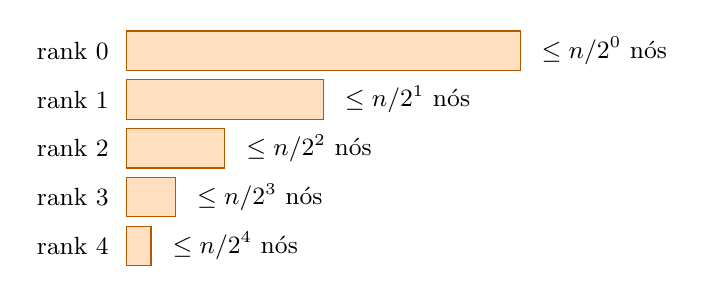
\begin{tikzpicture}
    \foreach \r in {0,1,2,3,4} {
      \pgfmathsetmacro{\w}{5/(2^\r)}
      \draw[fill=orange!25,draw=orange!70!black] (0,-0.62*\r) rectangle (\w,-0.62*\r+0.5);
      \node[anchor=east,font=\small] at (-0.1,-0.62*\r+0.25) {rank $\r$};
      \node[anchor=west,font=\small] at (\w+0.15,-0.62*\r+0.25) {$\leq n/2^{\r}$ nós};
    }
  \end{tikzpicture}

  \medskip
  \raggedright
  É uma \textbf{pirâmide}: metade dos nós tem rank baixo, e os ranks altos
  são raros.  Em particular, os nós de rank maior que $j$ são no máximo
  $n/2^j$.
\end{frame}

% ===================================================================
\begin{frame}[t]{Análise (2/3): agrupar os ranks em faixas}
  \small
  Dividimos os ranks possíveis ($0,\dots,\log_2n$) em \textbf{faixas}
  que ficam cada vez mais largas: a faixa $g$ cobre os ranks
  $(K,2^K]$, com $K$ o fim da faixa anterior.

  \medskip
  \centering
  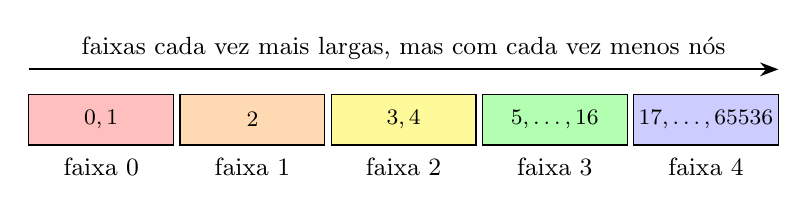
\begin{tikzpicture}[scale=.8]
    \foreach \x/\lab/\c/\g in {0/{$0,1$}/red!25/0, 2.4/{$2$}/orange!30/1,
        4.8/{$3,4$}/yellow!40/2, 7.2/{$5,\dots,16$}/green!30/3,
        9.6/{$17,\dots,65536$}/blue!20/4} {
      \draw[fill=\c] (\x,0) rectangle (\x+2.3,0.8);
      \node[font=\footnotesize] at (\x+1.15,0.4) {\lab};
      \node[font=\small] at (\x+1.15,-0.35) {faixa \g};
    }
    \draw[->,thick] (0,1.2) -- (11.9,1.2) node[midway,above,font=\small]
      {faixas cada vez mais largas, mas com cada vez menos nós};
  \end{tikzpicture}

  \medskip
  \raggedright
  A largura \textbf{explode} (de $K$ para $2^K$), então bastam
  $\lgs n$ faixas para cobrir todos os ranks.  \textbf{Compromisso:}
  faixa mais larga $\Rightarrow$ cada nó pode pagar mais vezes, mas a
  pirâmide garante que há menos nós nela.
\end{frame}

% ===================================================================
\begin{frame}[t]{Análise (3/3): quem paga cada busca?}
  \small
  Numa busca, um nó $y$ do caminho paga $O(1)$.  Separamos os pagantes:

  \medskip
  \begin{block}{Tipo 1: a raiz, o filho da raiz, ou quem \textbf{troca de faixa} para o pai}
    No caminho o rank só cresce, então o caminho cruza no máximo
    $\lgs n$ faixas: \textbf{$\leq\lgs n+1$ nós por busca}, em
    $O(m\lgs n)$ ao todo.
  \end{block}

  \begin{block}{Tipo 2: $y$ e o pai estão na \textbf{mesma} faixa}
    Cada vez que $y$ paga, ele passa a apontar para a raiz, que tem rank
    \textbf{maior} que o do pai anterior.  Como a faixa tem no máximo
    $2^K$ ranks, $y$ paga no máximo $2^K$ vezes e depois seu pai sai da
    faixa.  A faixa tem no máximo $n/2^K$ nós:
    \[
      \underbrace{\frac{n}{2^K}}_{\text{nós}}\cdot
      \underbrace{2^K}_{\text{pagamentos}}=n
      \qquad\Rightarrow\qquad \text{cada faixa custa }n.
    \]
    Com $\lgs n$ faixas: $O(n\lgs n)$.
  \end{block}
\end{frame}

% ===================================================================
\begin{frame}[t]{Resumo}
  \small
  \centering
  \renewcommand{\arraystretch}{1.5}
  \begin{tabular}{|l|l|c|}\hline
    \textbf{Estrutura} & \textbf{Quem paga e quanto} &
    \textbf{$m$ operações} \\ \hline\hline
    Vetor & cada união paga $n$ & $O(m+n^2)$ \\ \hline
    Listas, menor lista & cada elemento paga $\leq\log n$ & $O(m+n\log n)$ \\ \hline
    Floresta (tam./altura) & cada busca paga $\leq\log n$ & $O(m(1+\log n))$ \\ \hline
    Floresta + compressão & cada faixa de rank paga $n$ &
    $O((m+n)\lgs n)$ \\ \hline
  \end{tabular}

  \medskip\normalsize
  No Kruskal, com $m=O(|E|)$ e $n=|V|$, as três últimas deixam a
  ordenação das arestas, $O(|E|\log|V|)$, como o termo dominante.
\end{frame}

% ===================================================================
\appendix
\begin{frame}[plain]
  \centering\Large
  Apêndice\\[1ex]
  \normalsize Demonstrações formais
\end{frame}

\begin{frame}[t]{Listas ligadas: a heurística da menor lista}
  \small
  \begin{block}{Atualizar sempre a menor lista \hfill $(\ddag)$}
    Numa união, os ponteiros $\mathtt{rep}$ são atualizados na menor das
    duas listas (em qualquer uma, se têm o mesmo tamanho), que é
    acrescentada ao final da maior; isto é, a menor lista faz o papel de
    $L_y$ na descrição de $\Uniao$.
  \end{block}

  \medskip
  \textit{Intuição:} cada vez que $\mathtt{rep}[x]$ é atualizado, a
  lista de $x$ pelo menos dobra de tamanho.

  \begin{block}{Proposição}
    Supondo $(\ddag)$, em qualquer momento, se $\mathtt{rep}[x]$ foi
    atualizado $k$ vezes, então a lista que contém $x$ tem pelo menos
    $2^k$ elementos.
  \end{block}
  \begin{proof}[Prova]
    \footnotesize
    Os conjuntos só crescem, logo o tamanho da lista de $x$ não diminui.
    Indução em $k$: para $k=0$, a lista tem pelo menos $1=2^0$ elemento.
    Seja $k\geq1$ e $L$ a lista de $x$ imediatamente antes da $k$-ésima
    atualização; por indução e monotonicidade, $|L|\geq2^{k-1}$.  Como
    $\mathtt{rep}[x]$ é atualizado, por $(\ddag)$ a outra lista $L'$
    tem $|L'|\geq|L|$, e a lista resultante tem
    $|L|+|L'|\geq2|L|\geq2^k$ elementos.
  \end{proof}
\end{frame}

\begin{frame}[t]{União por tamanho: tamanho $\times$ altura}
  \small
  \begin{block}{Proposição}
    Usando união por tamanho, e supondo que as $n$ primeiras operações
    são $\Cria$, em qualquer momento cada árvore tem pelo menos $2^h$
    nós, onde $h$ é a sua altura.
  \end{block}
  \begin{proof}[Prova]
    \footnotesize
    Indução no número $k$ de uniões já realizadas.  Para $k=0$, as
    únicas operações até então que alteram a estrutura são $\Cria$, e
    toda árvore tem um nó e altura $0$, com $1\geq2^0$.  Seja $k\geq1$:
    como as $n$ primeiras operações são $\Cria$, nada além das uniões
    altera a estrutura.  A $k$-ésima união liga duas árvores distintas
    $A$ e $B$, com tamanhos $t_A,t_B$ e alturas $h_A,h_B$; por indução
    $t_A\geq2^{h_A}$ e $t_B\geq2^{h_B}$.  Sem perda de generalidade
    $t_A\geq t_B$ e a raiz de $B$ é pendurada na de $A$.  A árvore
    resultante tem $t'=t_A+t_B$ nós e altura $h'=\max\{h_A,h_B+1\}$.
    \begin{itemize}
    \item Se $h'=h_A$: $t'\geq t_A\geq2^{h_A}=2^{h'}$.
    \item Se $h'=h_B+1$: $t'=t_A+t_B\geq2t_B\geq2\cdot2^{h_B}=2^{h'}$.
    \end{itemize}
  \end{proof}
\end{frame}
% ==============================================================
\begin{frame}[t]{Um resultado mais fraco: grupos de \textit{rank}}
  \small
  Considere $m$ operações, as $n$ primeiras $\Cria$, com união por
  \textit{rank} e compressão.  Sejam $b_0=1$ e $b_g=2^{b_{g-1}}$, isto
  é, $1,2,4,16,65536,\dots$

  Particionamos $\mathcal U$ em \textbf{grupos} segundo o \textit{rank
    final}:
  \begin{itemize}
  \item Grupo $0$: elementos de rank $0$ e $1$;
  \item Grupo $g\geq1$: elementos de rank em $(b_{g-1},b_g]=(K,2^K]$,
    com $K=b_{g-1}$.
  \end{itemize}
  \begin{block}{Propriedades do \textit{rank}}
    \begin{enumerate}[(i)]
    \item o rank de um nó só muda em $\Link$, quando ele é a raiz que
      recebe a outra; depois que deixa de ser raiz, não muda mais;
    \item $\mathrm{rank}[x]<\mathrm{rank}[\mathrm{pai}[x]]$ para todo
      $x$ que não é raiz; em particular, $\mathrm{rank}[\mathrm{pai}[x]]$
      não decresce ao longo do tempo, e aumenta estritamente quando a
      compressão passa a apontar $x$ para um novo pai;
    \item se $x\neq y$ têm o mesmo rank final, então
      $D(x)\cap D(y)=\emptyset$, e $|D(x)|\geq2^{\mathrm{rank}[x]}$,
      onde $D(x)$ é a árvore de $x$ no instante em que $x$ deixa de ser
      raiz (ou no fim);
    \item para todo inteiro $j\geq0$, há no máximo $n/2^j$ nós de rank
      maior que $j$; em particular (com $j=K=b_{g-1}$), o Grupo $g$ tem
      no máximo $n/2^K$ nós;
    \item há no máximo $\lgs n$ grupos.
    \end{enumerate}
  \end{block}
\end{frame}

\begin{frame}[t]{Justificativa de (ii) e (iii)}
  \footnotesize
  \textbf{(ii)} Vale na criação; em $\Link$, se os ranks são iguais o da
  raiz que recebe aumenta; e a compressão aponta $x$ para um ancestral, que
  tem rank maior por transitividade de (ii) ao longo do caminho até a
  raiz.  Logo $\mathrm{rank}[\mathrm{pai}[x]]$ não decresce.

  \medskip
  \textbf{(iii)} A árvore de $x$ no instante em que deixa de ser raiz
  tem pelo menos $2^{\mathrm{rank}[x]}$ nós (proposição com rank), e o
  seu rank já é o final por (i).

  Suponha $z\in D(x)\cap D(y)$, com $x\neq y$ do mesmo rank $r$ e, sem
  perda de generalidade, $x$ deixando de ser raiz antes de $y$ (ou $y$
  sendo raiz no fim).
  \begin{itemize}
  \item Nesse instante $x$ é ligado a uma raiz $R$ de rank $\geq r$;
    após o $\Link$ a raiz da árvore de $z$ passa a ter rank $>r$ (se
    $\mathrm{rank}[R]=r$, ele aumenta), e esse rank não decresce.
  \item Quando $y$ deixa de ser raiz, $y$ é a raiz da árvore de $z$ com
    rank $r$: contradição.
  \end{itemize}
\end{frame}

\begin{frame}[t]{Justificativa de (iv) e (v)}
  \footnotesize
  \textbf{(iv)} Para cada $r$, os $D(x)$ de rank $r$ são disjuntos e têm
  $\geq2^r$ elementos, logo há $\leq n/2^r$ nós de rank $r$.  Somando
  sobre $r>j$:
  \[
    \sum_{r>j}\frac{n}{2^r}=\frac{n}{2^j}.
  \]

  \medskip
  \textbf{(v)} O rank é no máximo $\lfloor\lg n\rfloor$ (proposição).
  Se $g_0$ é o menor $g$ com $b_g\geq\lfloor\lg n\rfloor$, há $g_0+1$
  grupos.  Para $g_0\geq1$ vale $b_{g_0-1}<\lg n$, isto é,
  $n>2^{b_{g_0-1}}=b_{g_0}$.  Aplicando $\lg$ repetidamente,
  \[
    \lg^{(g_0)}n>\lg^{(g_0)}b_{g_0}=b_0=1,
  \]
  logo $\lgs n\geq g_0+1$.
\end{frame}

\begin{frame}[t]{Custo das buscas: nós de dois tipos}
  \small
  O custo total é $O(m)$ ($\Cria$ e $\Link$ custam $O(1)$) mais o custo
  das $f\leq2m$ buscas.  O custo de uma busca é o número de nós do
  caminho $x=y_0,\dots,y_k$ até a raiz, cujos apontadores são
  redirecionados.  Classificamos os nós $y$ do caminho:
  \begin{enumerate}
  \item \textbf{Tipo 1:} $y$ é a raiz ou filho da raiz, ou
    $\mathrm{pai}[y]$ está em grupo diferente do de $y$;
  \item \textbf{Tipo 2:} os demais, isto é, $y$ não é a raiz nem filho
    da raiz e $\mathrm{pai}[y]$ está no mesmo grupo que $y$.
  \end{enumerate}

  \medskip
  \begin{block}{Tipo 1}
    Ao longo do caminho o rank cresce estritamente, logo o grupo não
    decresce e muda no máximo $\lgs n-1$ vezes; com a raiz e o filho da
    raiz, cada busca tem no máximo $\lgs n+1$ nós do Tipo 1.  Em $f$
    buscas são
    \[
      O(m\lgs n).
    \]
  \end{block}
\end{frame}

\begin{frame}[t]{Nós do Tipo 2}
  \small
  Seja $y$ no Grupo $g\geq1$, com ranks em $(K,2^K]$.  Cada vez que $y$
  é do Tipo 2 em uma busca, $\mathrm{pai}[y]$ passa a ser a raiz, cujo
  rank é maior que o do pai anterior (pois este não era a raiz).  Como o
  rank do pai não decresce e o de $y$ é fixo por (i):
  \begin{itemize}
  \item o rank de $\mathrm{pai}[y]$ assume valores distintos em
    $(\mathrm{rank}[y],2^K]$ a cada ocorrência;
  \item depois que sai do grupo, $y$ nunca mais é do Tipo 2.
  \end{itemize}
  Logo $y$ é do Tipo 2 no máximo $2^K$ vezes.  Por (iv) há no máximo
  $n/2^K$ tais nós, e o Grupo $g$ contribui com no máximo
  \[
    \frac{n}{2^K}\cdot2^K=n.
  \]
  No Grupo $0$ cada nó é do Tipo 2 no máximo uma vez (o pai precisa ter
  rank $1$, e depois o pai passa para fora do grupo): contribui com no
  máximo $n$.  Somando sobre os $\leq\lgs n$ grupos,
  \[
    O(n\lgs n).
  \]
\end{frame}

\end{document}

%%% Local Variables:
%%% mode: LaTeX
%%% TeX-master: t
%%% End:
